\documentclass[a4paper]{article}
%\usepackage[singlespacing]{setspace}
\usepackage[onehalfspacing]{setspace}
%\usepackage[doublespacing]{setspace}
\usepackage{geometry} % Required for adjusting page dimensions and margins
\usepackage{amsmath,amsfonts,stmaryrd,amssymb,mathtools,dsfont} % Math packages
\usepackage{tabularx}
\usepackage{colortbl}
\usepackage{listings}
\usepackage{amsmath}
\usepackage{amssymb}
\usepackage{enumerate}
\usepackage{enumitem}
\usepackage{amsthm}
\usepackage{subcaption}
\usepackage{float}
\usepackage[table,xcdraw]{xcolor}
\usepackage{tikz-qtree}
\usepackage{forest}
\usepackage{changepage,titlesec,fancyhdr} % For styling Header and Titles
\pagestyle{fancy}
\renewcommand{\headrulewidth}{0.5pt} % Linienbreite anpassen, falls gewünscht
\renewcommand{\headrule}{
    \makebox[\textwidth]{\rule{1.0\textwidth}{0.5pt}} 
}
\usepackage{amsmath}
\pagestyle{fancy}
\usepackage{diagbox}
\usepackage{xfrac}

\usepackage{pgfplots}
\usepackage{pgfplotstable}
\pgfplotsset{compat=1.18}

\usepackage{enumerate} % Custom item numbers for enumerations

\usepackage[ruled]{algorithm2e} % Algorithms

\usepackage[framemethod=tikz]{mdframed} % Allows defining custom boxed/framed environments

\usepackage{listings} % File listings, with syntax highlighting
\lstset{
	basicstyle=\ttfamily, % Typeset listings in monospace font
}

\usepackage[ddmmyyyy]{datetime}


\geometry{
	paper=a4paper, % Paper size, change to letterpaper for US letter size
	top=3cm, % Top margin
	bottom=3cm, % Bottom margin
	left=2.5cm, % Left margin
	right=2.5cm, % Right margin
	headheight=25pt, % Header height
	footskip=1.5cm, % Space from the bottom margin to the baseline of the footer
	headsep=1cm, % Space from the top margin to the baseline of the header
	%showframe, % Uncomment to show how the type block is set on the page
}
\lhead{\vspace{0.5\baselineskip}Übungsblatt 4}
\chead{\bfseries{Einführung in Verteilte Systeme\\Sommersemester 2025}}
\rhead{\vspace{0.5\baselineskip}Werner, 7987847}
\fancyheadoffset[R]{0cm}

\begin{document}
\setcounter{section}{4}
\subsection{}
Gegeben sei das folgende Non-Return-to-Zero-kodierte Signal:\\
\begin{center}
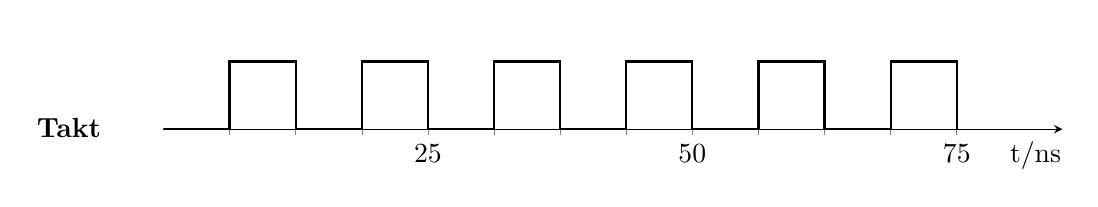
\begin{tikzpicture}
    \node at (-1.2,0.45) {\textbf{Takt}};
      \begin{axis}[
        axis lines=middle,
        xlabel={t/ns},
        xlabel style={at={(axis description cs:0.97,0.23)}, anchor=north},
        y axis line style={draw=none},
        ylabel={\empty},
        xtick={0,6.25,...,75},
        xticklabels={
          0, , , ,
          25, , , ,
          50, , , ,
          75,
        },
        ytick=\empty,
        width=13cm,
        height=3.3cm,
        ymin=-0.5, ymax=1.5,
        xmin=0, xmax=85,
        enlargelimits=false,
        domain=0:12,
        samples=100,
      ]
      \addplot[
        black,
        thick
      ] coordinates {
          (0,0)
          (6.25,0)
          (6.25,1)
          (12.5,1)
          (12.5,0)
          (18.75,0)
          (18.75,1)
          (25,1)
          (25,0)
          (31.25,0)
          (31.25,1)
          (37.5,1)
          (37.5,0)
          (43.75,0)
          (43.75,1)
          (50,1)
          (50,0)
          (56.25,0)
          (56.25,1)
          (62.5,1)
          (62.5,0)
          (68.75,0)
          (68.75,1)
          (75,1)
          (75,0)
    };
    \end{axis}
\end{tikzpicture}
\end{center}

\begin{center}
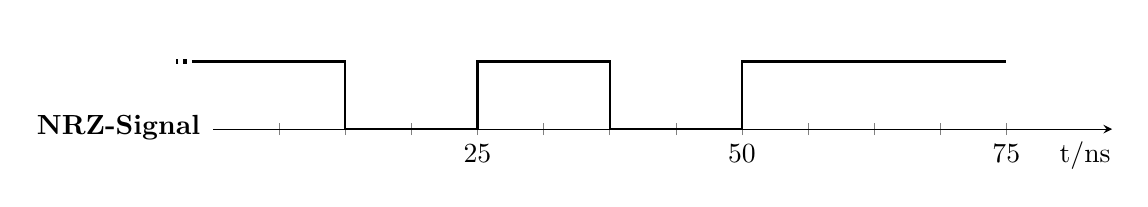
\begin{tikzpicture}
    \node at (-1.2,0.45) {\textbf{NRZ-Signal}};
      \begin{axis}[
        axis lines=middle,
        xlabel={t/ns},
        xlabel style={at={(axis description cs:0.97,0.23)}, anchor=north},
        y axis line style={draw=none},
        ylabel={\empty},
        xtick={0,6.25,...,75},
        xticklabels={
          0, , , ,
          25, , , ,
          50, , , ,
          75,
        },
        ytick=\empty,
        width=13cm,
        height=3.3cm,
        ymin=-0.5, ymax=1.5,
        xmin=0, xmax=85,
        enlargelimits=false,
        clip=false,
        domain=0:12,
        samples=100,
      ]
      \addplot[
        black,
        thick
      ] coordinates {
          (-2,1)
          (12.5,1)
          (12.5,0)
          (25,0)
          (25,1)
          (37.5,1)
          (37.5,0)
          (50,0)
          (50,1)
          (62.5,1)
          (75,1)
    };

    \addplot[
        black,
        line width=1.5pt,
        dash pattern=on 1.2pt off 1.8pt
      ] coordinates {
          (-2.5,1)
          (-3.5,1)
    };
    \end{axis}
\end{tikzpicture}
\end{center}

\noindent Im Folgenden soll NRZI in der NRZI-M-Kodierung verwendet werden, so dass sich jeweils ein Zustandswechsel bei einem Eins-Bit ergibt.
\begin{enumerate}[label=\alph*)]
    \item Dekodieren Sie die in dem dargestellten NRZ-Signal übertragenen Bits.\\
    $\Rightarrow$ \textbf{101011}
    \item Bestimmen Sie die Bitrate des dargestellten NRZ-Signals in Mbit/s.\\
    \[\frac{\text{Codelänge (Bitanzahl)}}{\text{Gesamtübermittlungsdauer}}\frac{6\, bit}{75\, ns}=0,08\, bit/ns = 80\, Mbit/s\]
    \item Zeichnen Sie das NRZI-Signal, das der gegebenen Bitfolge entspricht.\\
    \begin{center}
    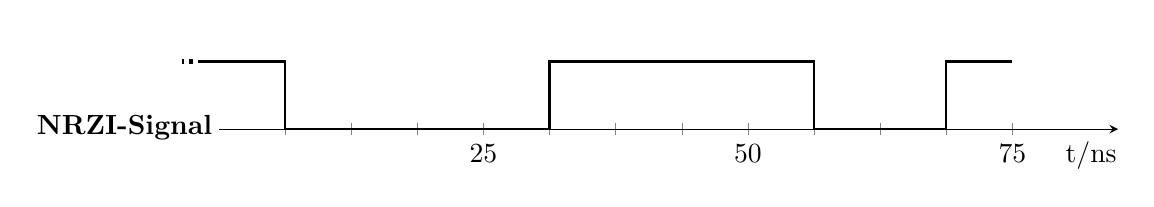
\begin{tikzpicture}
    \node at (-1.2,0.45) {\textbf{NRZI-Signal}};
      \begin{axis}[
        axis lines=middle,
        xlabel={t/ns},
        xlabel style={at={(axis description cs:0.97,0.23)}, anchor=north},
        y axis line style={draw=none},
        ylabel={\empty},
        xtick={0,6.25,...,75},
        xticklabels={
          0, , , ,
          25, , , ,
          50, , , ,
          75,
        },
        ytick=\empty,
        width=13cm,
        height=3.3cm,
        ymin=-0.5, ymax=1.5,
        xmin=0, xmax=85,
        enlargelimits=false,
        clip=false,
        domain=0:12,
        samples=100,
      ]
      \addplot[
        black,
        thick
      ] coordinates {
          (-2,1)
          (6.25,1)
          (6.25,0)
          (31.25,0)
          (31.25,1)
          (56.25,1)
          (56.25,0)
          (68.75,0)
          (68.75,1)
          (75,1)
    };

    \addplot[
        black,
        line width=1.5pt,
        dash pattern=on 1.2pt off 1.8pt
      ] coordinates {
          (-2.5,1)
          (-3.5,1)
    };
    \end{axis}
    \end{tikzpicture}
    \end{center}
    \item Takt-Rückgewinnung: Kann ein NRZI-Signal alleine verwendet werden, um die Information zu übertragen, oder muss ein Taktsignal zur Synchronisation mitgesendet werden?\\
    Begründen Sie Ihre Antwort in einem Satz. \\\\
    Nein, ohne eine Taktfrequenz oder Taktsignal kann das Signal nicht zuverlässig dekodiert werden. Längere konstante Intervalle bieten nicht genügend Flanken um eine Taktfrequenz zu erschließen.
\end{enumerate}
\clearpage 
\subsection{}
\begin{enumerate}[label=\alph*)]
    \item Dekodieren Sie das dargestellte Manchester-kodierte Signal.\\
    (Es gilt, analog zur Vorlesung, folgende Definition: Ein $0 \to 1$-Übergang sei eine logische Null, $1 \to 0$ eine logische Eins.)\\
    \begin{center}
    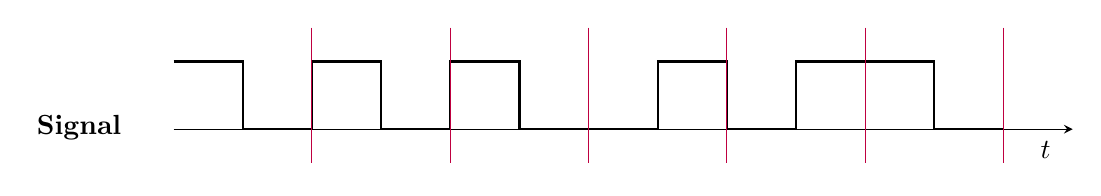
\begin{tikzpicture}
    \node at (-1.2,0.45) {\textbf{Signal}};
      \begin{axis}[
        axis lines=middle,
        xlabel={$t$},
        xlabel style={at={(axis description cs:0.97,0.23)}, anchor=north},
        y axis line style={draw=none},
        ylabel={\empty},
        xtick={\empty},
        ytick=\empty,
        width=13cm,
        height=3.3cm,
        ymin=-0.5, ymax=1.5,
        xmin=0, xmax=13,
        enlargelimits=false,
        domain=0:12,
        samples=100,
      ]
      \addplot[
        black,
        thick
      ] coordinates {
        (0,1)
        (1,1)
        (1,0)
        (2,0)
        (2,1)
        (3,1)
        (3,0)
        (4,0)
        (4,1)
        (5,1)
        (5,0)
        (6,0)
        (7,0)
        (7,1)
        (8,1)
        (8,0)
        (9,0)
        (9,1)
        (11,1)
        (11,0)
        (12,0)
      };
      \addplot[purple] coordinates {(2,1.5) (2,-0.5)};
    \addplot[purple] coordinates {(4,1.5) (4,-0.5)};
    \addplot[purple] coordinates {(6,1.5) (6,-0.5)};
    \addplot[purple] coordinates {(8,1.5) (8,-0.5)};
    \addplot[purple] coordinates {(10,1.5) (10,-0.5)};
    \addplot[purple] coordinates {(12,1.5) (12,-0.5)};
      \end{axis}
    \end{tikzpicture}
    \end{center}
    \vspace*{-1cm}
    \begin{center}
    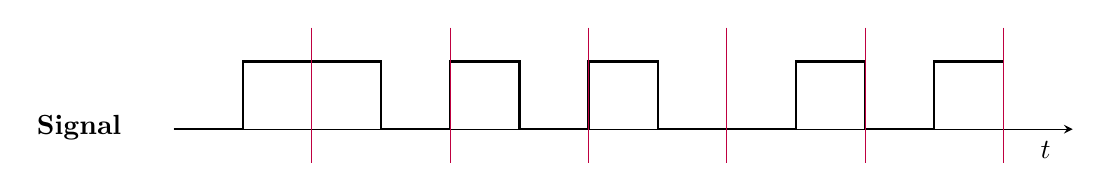
\begin{tikzpicture}
    \node at (-1.2,0.45) {\textbf{Signal}};
      \begin{axis}[
        axis lines=middle,
        xlabel={$t$},
        xlabel style={at={(axis description cs:0.97,0.23)}, anchor=north},
        y axis line style={draw=none},
        ylabel={\empty},
        xtick={\empty},
        ytick=\empty,
        width=13cm,
        height=3.3cm,
        ymin=-0.5, ymax=1.5,
        xmin=0, xmax=13,
        enlargelimits=false,
        domain=0:12,
        samples=100,
      ]
      \addplot[
        black,
        thick
      ] coordinates {
        (0,0)
        (1,0)
        (1,1)
        (2,1)
        (2,1)
        (3,1)
        (3,0)
        (4,0)
        (4,1)
        (5,1)
        (5,0)
        (6,0)
        (6,1)
        (7,1)
        (7,0)
        (8,0)
        (9,0)
        (9,1)
        (10,1)
        (10,0)
        (11,0)
        (11,1)
        (12,1)
      };
      \addplot[purple] coordinates {(2,1.5) (2,-0.5)};
    \addplot[purple] coordinates {(4,1.5) (4,-0.5)};
    \addplot[purple] coordinates {(6,1.5) (6,-0.5)};
    \addplot[purple] coordinates {(8,1.5) (8,-0.5)};
    \addplot[purple] coordinates {(10,1.5) (10,-0.5)};
    \addplot[purple] coordinates {(12,1.5) (12,-0.5)};
      \end{axis}
    \end{tikzpicture}
    \end{center}
    Markieren Sie in der Abbildung die Grenzen zwischen übertragenen Bits mit vertikalen Strichen.\\
    \item Nun soll die Bitfolge 011100 übertragen werden. Zeichnen Sie den Verlauf des Manchesterkodierten Signals.
    \item Begründen Sie, ob sich dieses Manchesterkodierte Signal eindeutig bestimmen lässt.\\
    \begin{center}
    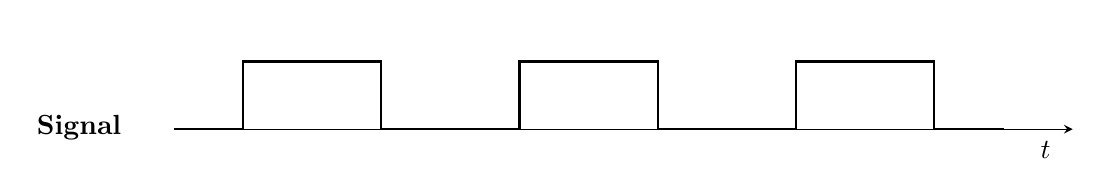
\begin{tikzpicture}
    \node at (-1.2,0.45) {\textbf{Signal}};Takt
      \begin{axis}[
        axis lines=middle,
        xlabel={$t$},
        xlabel style={at={(axis description cs:0.97,0.23)}, anchor=north},
        y axis line style={draw=none},
        ylabel={\empty},
        xtick={\empty},
        ytick=\empty,
        width=13cm,
        height=3.3cm,
        ymin=-0.5, ymax=1.5,
        xmin=0, xmax=13,
        enlargelimits=false,
        domain=0:12,
        samples=100,
      ]
      \addplot[
        black,
        thick
      ] coordinates {
        (0,0)
        (1,0)
        (1,1)
        (3,1)
        (3,0)
        (5,0)
        (5,1)
        (7,1)
        (7,0)
        (9,0)
        (9,1)
        (11,1)
        (11,0)
        (12,0)
      };
      \end{axis}
    \end{tikzpicture}
    \end{center}
    Ja, aus der Vorlesung wissen wir, dass Signale mit der Manchester-Kodierung eine Taktrückgewinnung ermöglichen. Durch die spezielle Kodierung gibt es pro Takt mindestens eine Flanke welche Orientierung und Synchronisierung bietet.
    \item Takt-Rückgewinnung: Kann das Manchester-Signal alleine verwendet werden, um die Information zu übertragen, oder muss ein Taktsignal zur Synchronisation mitgesendet werden?\\
    Begründen Sie Ihre Antwort in einem Satz\\\bigskip
    Ja, wie schon in der Teilaufgabe c) erwähnt, bietet die Manchester-Kodierung mindestens eine Flanke pro Takt, also für jedee Bitstelle, zur Eindeutigen Bestimmung des Signals. Somit erfolgt auch die Takt-Rückgewinnung, welche üblicherweise im 2. Schritt zur Bestimmung des Signals genutzt wird.
\end{enumerate}
\end{document}
